\documentclass[t,compress,11pt,xcolor=dvipsnames]{beamer}
\usefonttheme[onlymath]{serif}
\usetheme{Ilmenau}
\definecolor{LHCblue}{RGB}{4, 114, 255}
\usecolortheme[named=LHCblue]{structure}
\usepackage[bars]{beamerthemetree} % Beamer theme v 2.2
\usepackage{multicol}
\usepackage{lmodern}
\usepackage{lipsum}
\usepackage{marvosym}
\usepackage{hyperref}
\title{ CS251 Project Report by Group 12.}
\author[Pramod  \&  Basith \& Nikhileswar  ]
{
   \texorpdfstring{
        \begin{columns}
            \column{.30\linewidth}
            \centering
            Pramod \\
            140050076 \\
            {140050076@itb.ac.in}
            \column{.30\linewidth}
            \centering
            Basith \\
             140050070 \\
             {140050070@itb.ac.in}
            \column{.30\linewidth}
            \centering
            Nikhileswar \\
             140050074 \\
            {140050074@itb.ac.in}
        \end{columns}
   }
   {John Doe \& Jane Doe}
   }
\date{\today}

\begin{document}
\maketitle
\begin{frame}
\frametitle{Overview}
\tableofcontents
\end{frame}
\section{Introduction}
\begin{frame}
\frametitle{Introduction}
This report is made to describe the concepts behind our CS251 project Box2d simulation .\\~\\
We also would like to mention the references used to complete our project through this report.\\~\\
\end{frame}
%
\section{Motivation}
\begin{frame}
\frametitle{Motivation}
This project is a demonstration of the power of the software
systems like BOX2d .\\
A Rube Goldberg\cite{goldberg} machine is a contraption, invention, device or apparatus that is deliberately over-engineered to perform a simple task in a complicated fashion, usually including a chain reaction.\\
The basic concepts and machinery used in this can be utilized to generate even more complex and relevant games.\\
So we wish to build a Rube Goldberg Machine \cite{machine}  Simulation in which the balls are thrown into the basket in a complicated manner.  \\
This project involves several concepts discussed in this course like
makefile, doxygen,profiling, bash, beamer, libraries,html etc...\\
\end{frame}
\section{Aims}
\begin{frame}
\frametitle{Aims}
During the beggining of project our idea was to make this simulation and synchronize it such that both balls from left,right part of system collide. \\~\\
After completion of basic simulation we thought the whole purpose of the simulation was for nothing!!,so we added extra objects like dominos,revolving platforms to make it to do something.\\~\\
Finally the intial balls along with additional objects are  used to make all the 8balls fall into the basket type of system in the middle.\\~\\
The system simulation in left and right parts are in synchroniztion.Both the balls reach ground dominos same time.
\end{frame}
\section{Deviations}
\begin{frame}
\frametitle{Deviations}
The only deviation from our original plan was the failure to implement sccisors kind of object into our system.\\~\\
We tried by using cotactlistener function and then deleting the joints,but we got the basic idea but due to time bound we were unable to complete it.
\end{frame}
\section{Usage of previous labs}
\begin{frame}
\frametitle{Usage of previous labs}
We were successfull in using the previous labs during this project.
We used git,makefiles,doxygen,profiling,bash,html,latex,beamer(for reports)....\\~\\
\end{frame}
\section{Description}
\begin{frame}
\frametitle{Description}
\begin{columns}[t]
\column{0.3\textwidth}
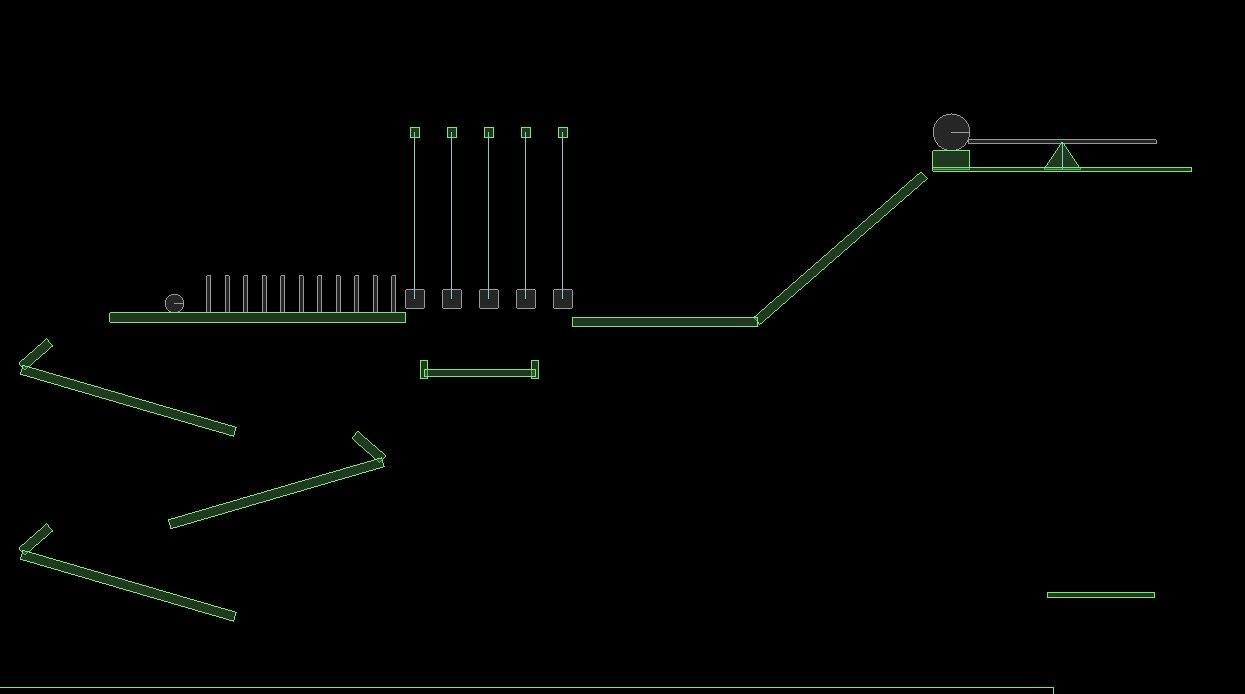
\includegraphics[width=4cm,height=3cm]{left.jpg}
\column{0.3\textwidth}
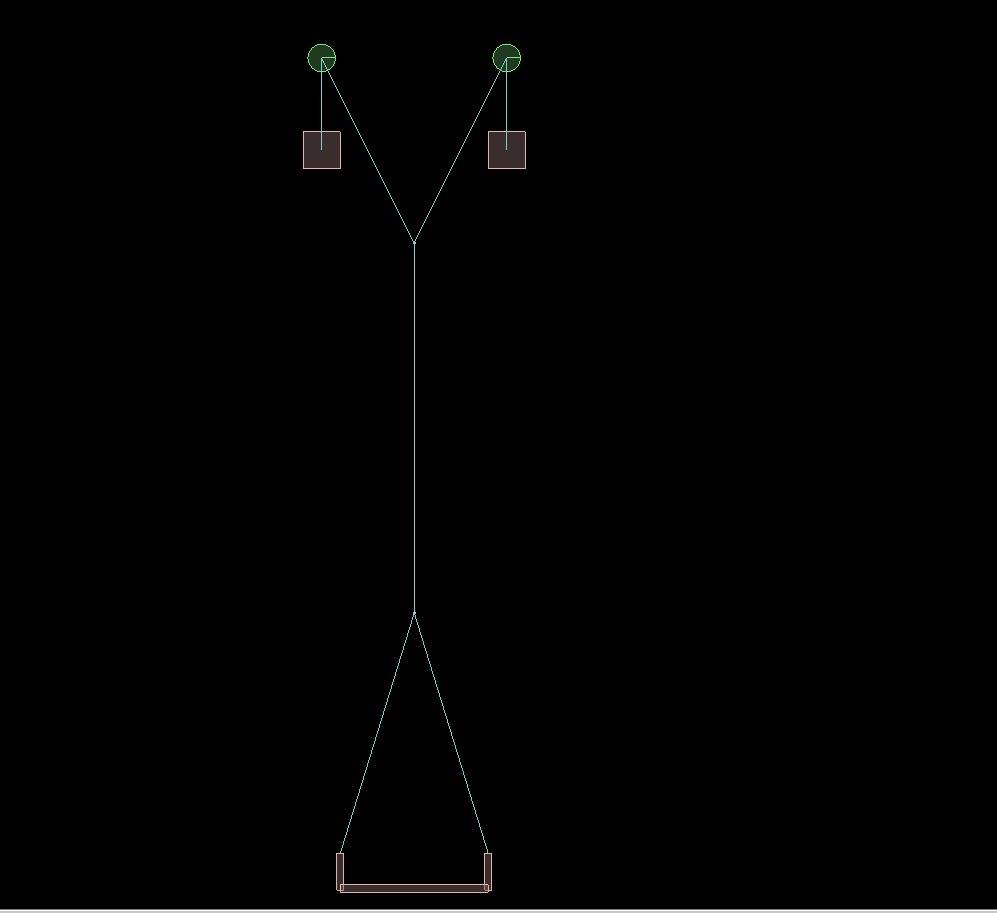
\includegraphics[width=4cm,height=3cm]{middle.jpg}
\column{0.4\textwidth}
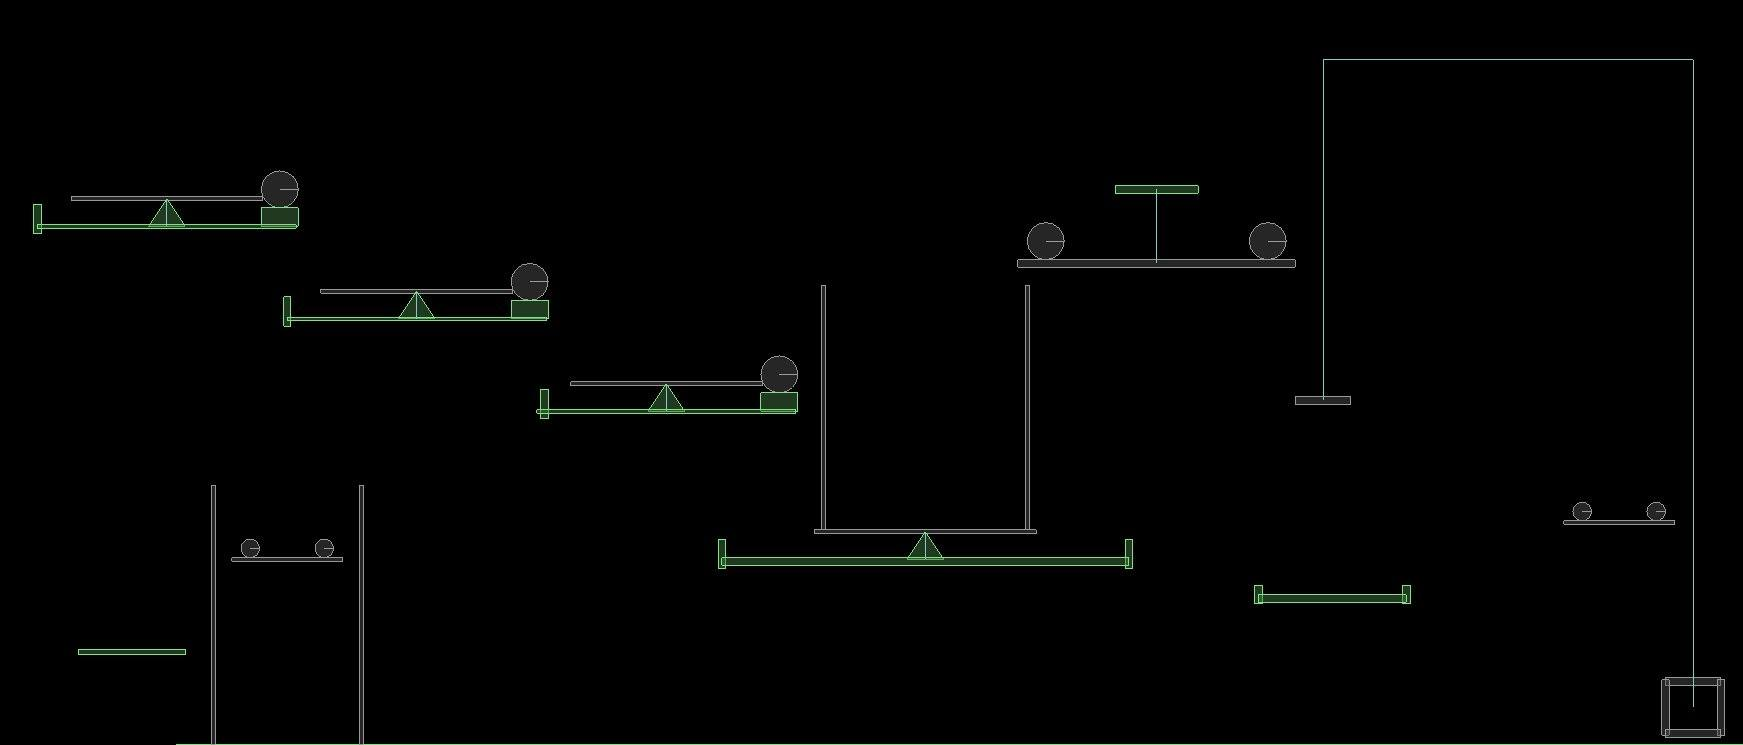
\includegraphics[width=4cm,height=3cm]{right.jpg}
\end{columns}
There are several objects in our project.We will briefly explain how  we created it alomg with its figure. \\~\\
\end{frame}
\begin{frame}
\frametitle{Inclined Planes}
\begin{center}

\includegraphics[width=4cm,height=3cm]{inclinedplanes}
\end{center}
We used few Inclined planes in the simulation.They are used in order to increase the momentum of the objects when objects pass along them.Beacuse the objects wont get required in x-direction if only horizontal planes are used when objects are allowed to fall through in gravity.
\end{frame}
\begin{frame}
\frametitle{Dominos}
\begin{columns}[t]
\column{0.5\textwidth}

\includegraphics[width=4cm,height=3cm]{dominos}
\column{0.5\textwidth}
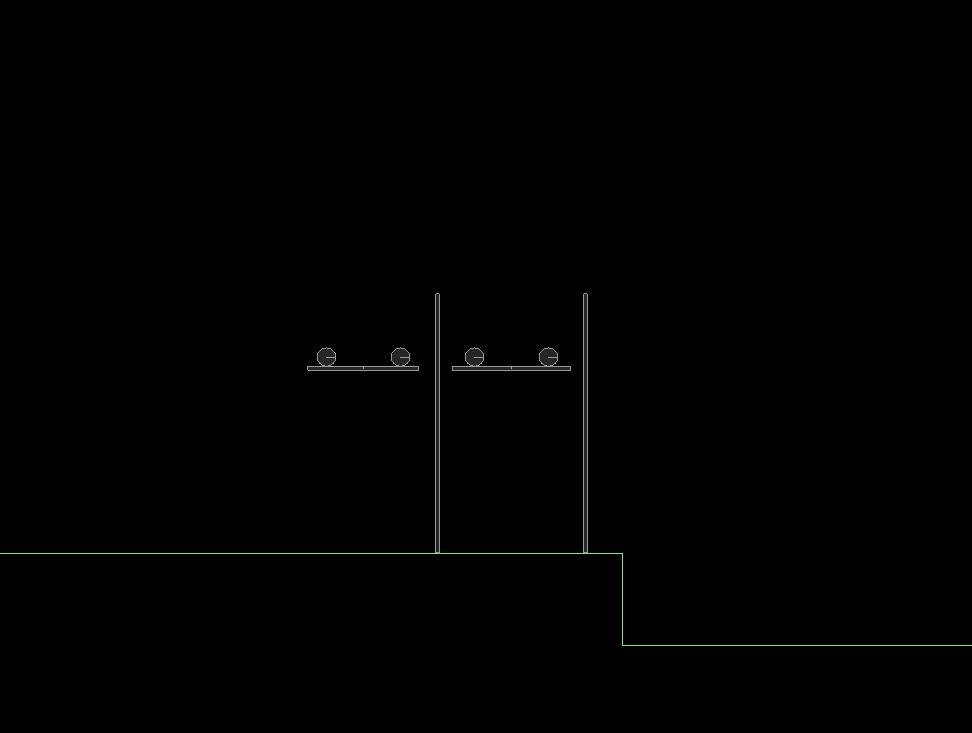
\includegraphics[width=4cm,height=3cm]{longdominos}
\end{columns}
We made it by placing a static platform and placing a small  dynamic rectangular blocks at regular intervals in such a way that if one of then falls remaining dominos will also fall.
\end{frame}
\begin{frame}
\frametitle{See-saw with Box and ball beside it}
\begin{center}

\includegraphics[width=4cm,height=3cm]{see-saw}
\end{center}
We made the simulation by creating a revolute joint between a static triangle and a dynamic rod,and placing a Box beside the plank.On the Box,a ball is placed.\\~\\
We arranged the system such that after ball hitting the one side of see-saw,the other side 
pushes the ball on the box which is beside the see-saw.
\end{frame}
\begin{frame}
\frametitle{See-saw with Two Long Dominoes on it}
\begin{center}
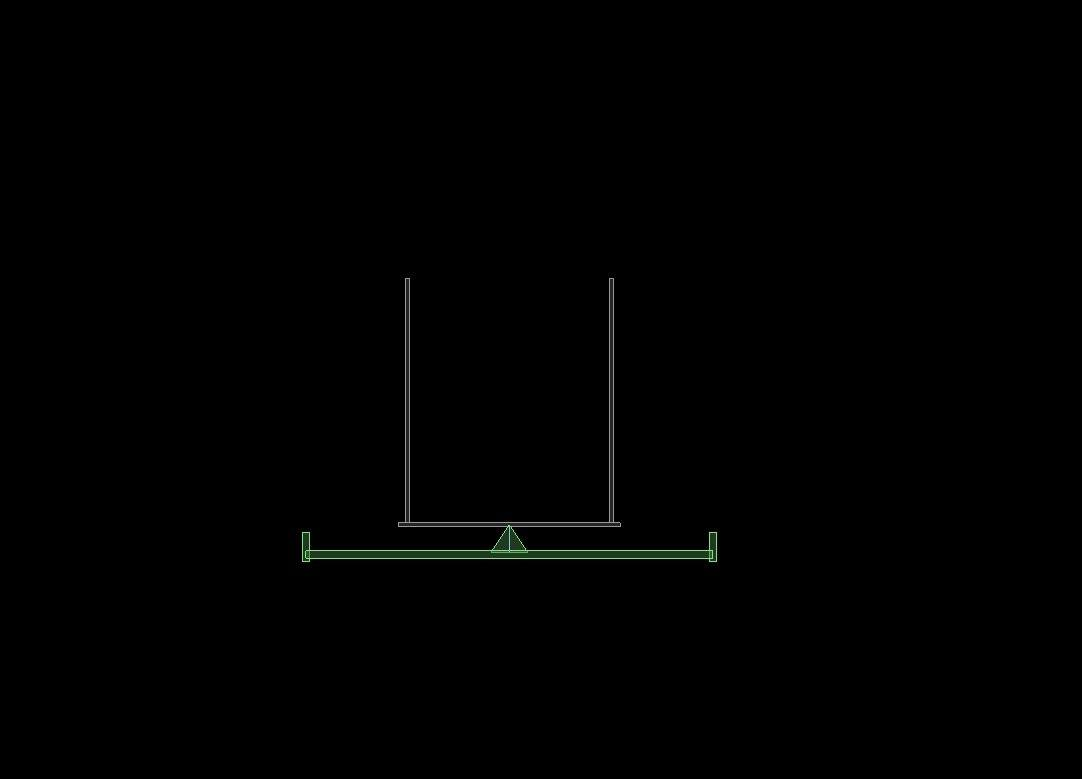
\includegraphics[width=4cm,height=3cm]{see-saw2}
\end{center}
We made the simulation by creating a revolute joint between a static triangle and a dynamic rod,and placing a long dominoes on two sides of the plank\\~\\
We arranged the system such that after ball hitting the other side of see-saw that block hits the hinged platform above it.
\end{frame}
\begin{frame}
\frametitle{REVOLVING PLATFORMS }
\begin{center}
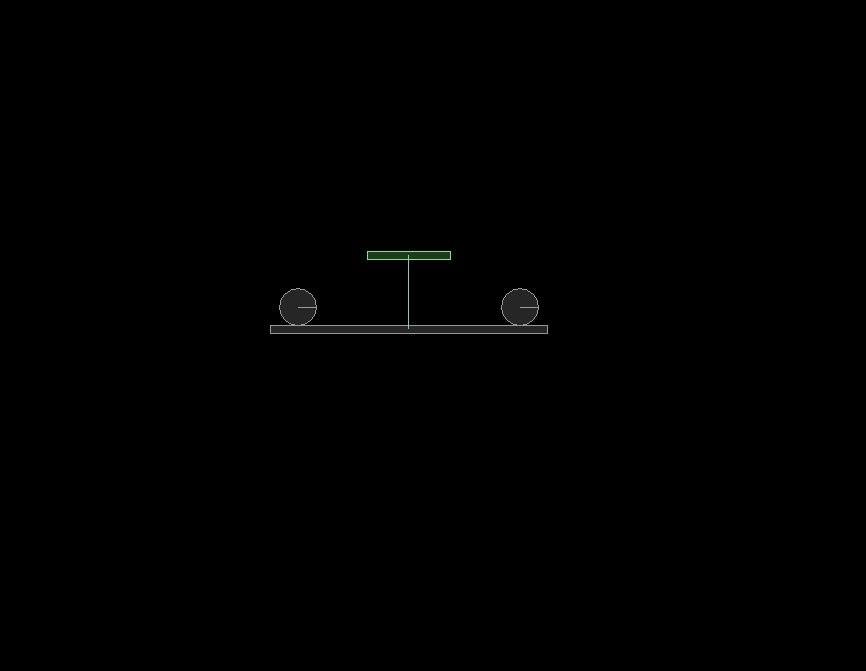
\includegraphics[width=4cm,height=3cm]{revolvingplatform}
\end{center}
We used Revolute Joint to make the effect of hinged rod.
It takes one anchors and two objects and connects the two objects with
the thread through the point.\\~\\
We defined one of the objects as a dynamic rod and other as a small
static object with the anchor point on itself which resulted in the effect
of this hinged rod
\end{frame}
\begin{frame}
\frametitle{RightPulley}
\begin{center}
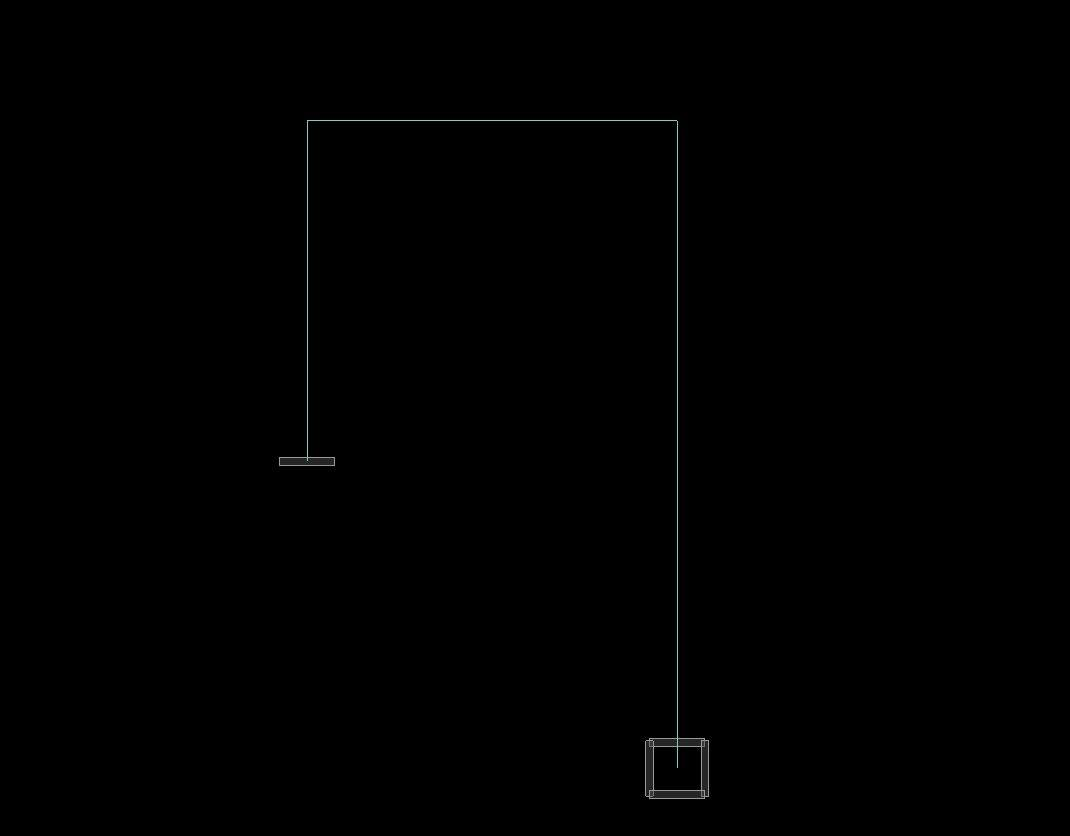
\includegraphics[width=5cm,height=4cm]{pulley}
\end{center}
We used PulleyJoint to make the pulleys.
It takes two objects and two points in world and two points on the objects.It connects the two objects through the two points.
We defined box and bar as the objects and their centers as anchor points on them,connected them through two points in the world. 
\end{frame}
\begin{frame}
\frametitle{Middle Pulley}
\begin{center}
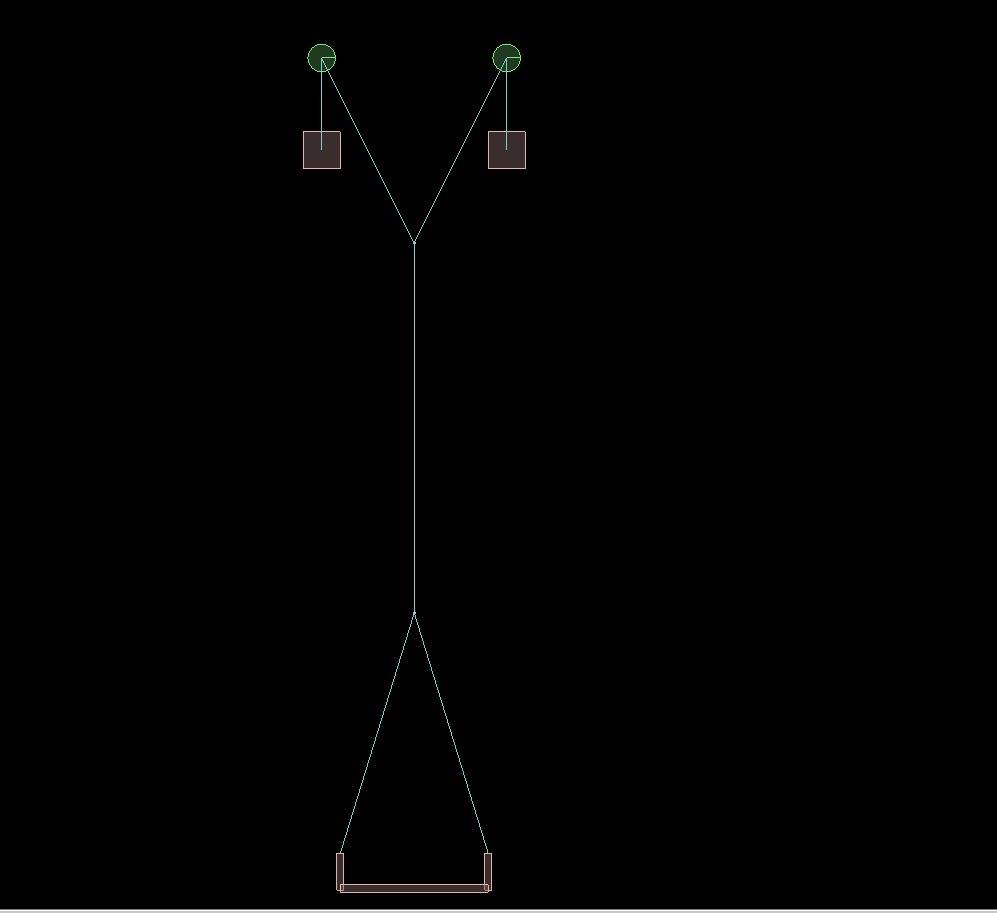
\includegraphics[width=8cm,height=6cm]{middlepulley}
\end{center}
\end{frame}
\begin{frame}
\frametitle{Middle Pulley}
We used PulleyJointDef and DistanceJoint to make this pulley.
DistanceJoint takes two objects and two points on it and creates thread between them.
We defined one of the objects as a dynamic box and other as a very small dynamic ball
with the two anchor points in the world being same,anchor points on box,small ball are their centers and used pulley joint to create top part of the middle pulley.
We defined one more small ball and connected with the above small ball using Distance joint.
We defined one open box and connected its each of its top ends with small box using Distance Joint.
\end{frame}
\begin{frame}
\frametitle{PENDULUM}
\begin{center}
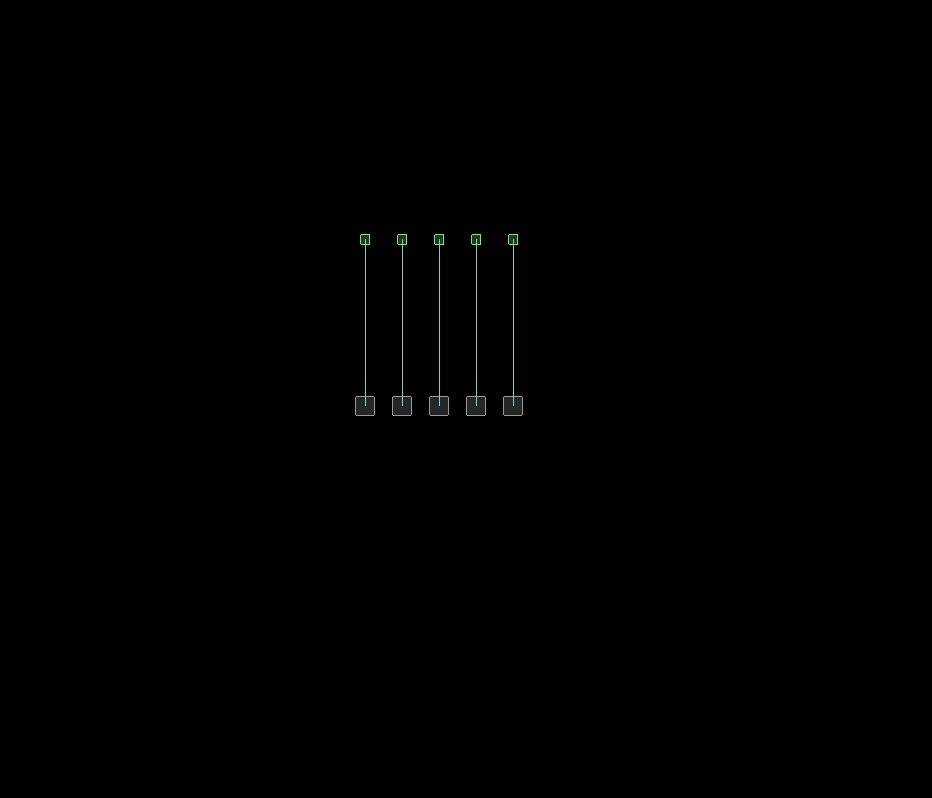
\includegraphics[width=4cm,height=3cm]{pendulum}
\end{center}
We used RevoluteJoint to create pendulums.
It is created using anchoring the thread such that the pendulum hits the dominos above it.
\end{frame}
\section{Profiling}
\begin{frame}
\frametitle{About Profiling}
Profing is very useful to write optimised programs.It gives the description of time consumed by different functions in our code so that we can understand which function to be optimised.
The flat profile of analysis.txt shows that all the function calls are taking vary less time.Therefore there is no need to optimise any particular function. However we user -O3 compiling option to optimise. The result of which is shown in analysis updated.txt .There we observe that the percentage of time for some of the function calls have increased which occurs because many of the functions have been optimised which can be known by checking the number of functions listed in the call graphs of both text files so the remaining time is distributed among the functions which results in the increased percentage oftime of those particular functions.
\end{frame}
\begin{frame}
\frametitle{Profiled output of Project}

\includegraphics[scale=.022]{output_updated.png}
\end{frame}
\begin{frame}
\frametitle{contributions}
Shaik AbdulBasith\cite{basith} :\\
Left Part Objects and some Right parts\\
Sinking and managing the three parts\\
PramodVakacharla\cite{pramod} :\\
Middle Parts\\
Gprof \\
Makefiles\\
Nikhileswar\cite{nikhileswar} :\\
Right Parts\\
Documenting\\
Latex\\

\end{frame}
\begin{frame}
\frametitle{Makefile Targets}
CodeDoc:\\
Completes Documentation\\
Report:\\
Compiles latex files and generates pdf files\\
Clean:\\
removes all the extra objects created\\
DistClean:
removes extra directories created\\
profile:\\
creates analysis.txt,analysis.dot,output.png\\
release:\\
sets up the box2D\\ 
\end{frame}
\bibliography{Report}
\bibliographystyle{plain}

\end{document}
